% !TeX root = ../main.tex

\chapter{Discussion}

In this chapter, we discuss the results we have seen in the previous chapter, and how they may echo with the research questions posed in Chapter \ref{chapter:Introduction}. Specifically, two main tenets are delved into: 1) tonal coarticulation in Taiwan Southern Min and Taiwan Mandarin, 2) interaction between strictness of tone boundaries and normalization for tonal coarticulation. In addition, we will also touch upon the issues regarding the nature of tonal coarticulation and of general versus speech-specific perception.

\section{Tonal coarticulation in Taiwan Mandarin and Taiwan Southern Min}

In this section, we talk about the coarticulatory effects of adjacent tones in Taiwan Mandarin and Taiwan Southern Min, and the consistencies as well as discrepancies between this and previous studies.

\subsection{Symmetric tonal coarticulation and final prominence}
As reviewed in Section \ref{section:Tonal coarticulation in Mandarin and Southern Min}, previous studies generally showed an asymmetry of Mandarin tonal coarticulation in both magnitude and directionality. A prevalent belief is that carry-over effects in Mandarin is stronger and assimilatory, while anticipatory effects are weaker and dissimilatory. While strong and assimilatory effects are also found in our data of Taiwan Mandarin, linear-mixed effect models did not show the anticipatory effects to be significantly weaker, and it was also found that these effects are assimilatory just as carry-over effects. This discrepancy of anticipatory effects between our and previous studies is particularly interesting. Comparison with Taiwan Southern Min may shed light on such finding. In both \cite{Peng1997} and this study, anticipatory effects were found to be assimilatory in Taiwan Southern Min. Such symmetry is likewise found in Malaysian Hokkien in \cite{ChangHsieh2012}, where the authors suggest that Southern Min and Hokkien as languages with rich sandhi rules, can be subject to final prominence, a feature that is of less importance in the previous investigated tonal languages where asymmetry exists in tonal coarticulation. It is argued in \cite{ChangHsieh2012} that the typological asymmetry in tonal coarticulation attested in literature may be likely due to the linearity of speech, which results in ``progressive bias'' and in turn favours rightward coarticulation over leftward anticipatory coarticulation. Such bias might be balanced in light of final prominence in Taiwan Southern Min/Malaysian Hokkien, resulting in rather similar distribution between the coarticulations of the two directions. Given the almost identical distributions of the data we have seen in Taiwan Mandarin and Taiwan Southern Min, one is propelled to believe that tonal coarticulation in Taiwan Mandarin might to a certain extent be under the influence of Taiwan Southern Min, and in turn leads to this dialectal difference we see between the data collected in this study and the results in previous researches of Mandarin, where the investigated dialects were all Beijing Mandarin. It is established that Taiwan Mandarin and Taiwan Southern Min as the two major languages in Taiwan, have profound interaction and mutual influence on virtually every linguistic level, including morphosyntax (e.g., \citealp{Li2008}) and phonlogy (e.g., \citealp{ChuangFon2010}; \citealp{Li2010}), and code-switching between the two languages are more than common in Taiwanese society (cf. \citealp{Yang2021}). Scholars including \cite{Her2012} and \cite{Su2018} also argues that Taiwan Mandarin is a highly unique localized variety of Mandarin, under the influence of Taiwan Southern Min and other Taiwanese languages\footnote{\citeauthor{Her2012} even goes as far to say Taiwan Mandarin is a new-born creole  unique to Taiwanese people.}. It is not inconceivable that Taiwan Mandarin might come under the influence of the final prominence we observe in Taiwan Southern Min and Malaysian Hokkien.

\subsection{Tone boundaries and perception of tonal coarticulation}\label{section:Tone boundaries and perception of tonal coarticulation}
Another issue that requires attention is the strong effect of tonal coarticulation we see in the Taiwan Southern Min data. As discussed in Chapter \ref{chapter:Introduction}, Taiwan Southern Min is a language with 7 lexical tones, with several of them contrasting with each other only in terms of tone value, and having the same tone shapes. This means that tone identification is a much harder task in Taiwan Southern Min than in Taiwan Mandarin. As can be seen in Fig. \ref{Figure:ToneSpace}, if we plot the tone onsets and offsets of the tones produced in isolation by the subjects, the 95\% confidence intervals largely overlap with each other in Taiwan Southern Min. One might imagine these to be even messier when the tones are coarticulated.
\begin{figure}[hbt!]
\centering
\begin{subfigure}[b]{.8\textwidth}
\centering
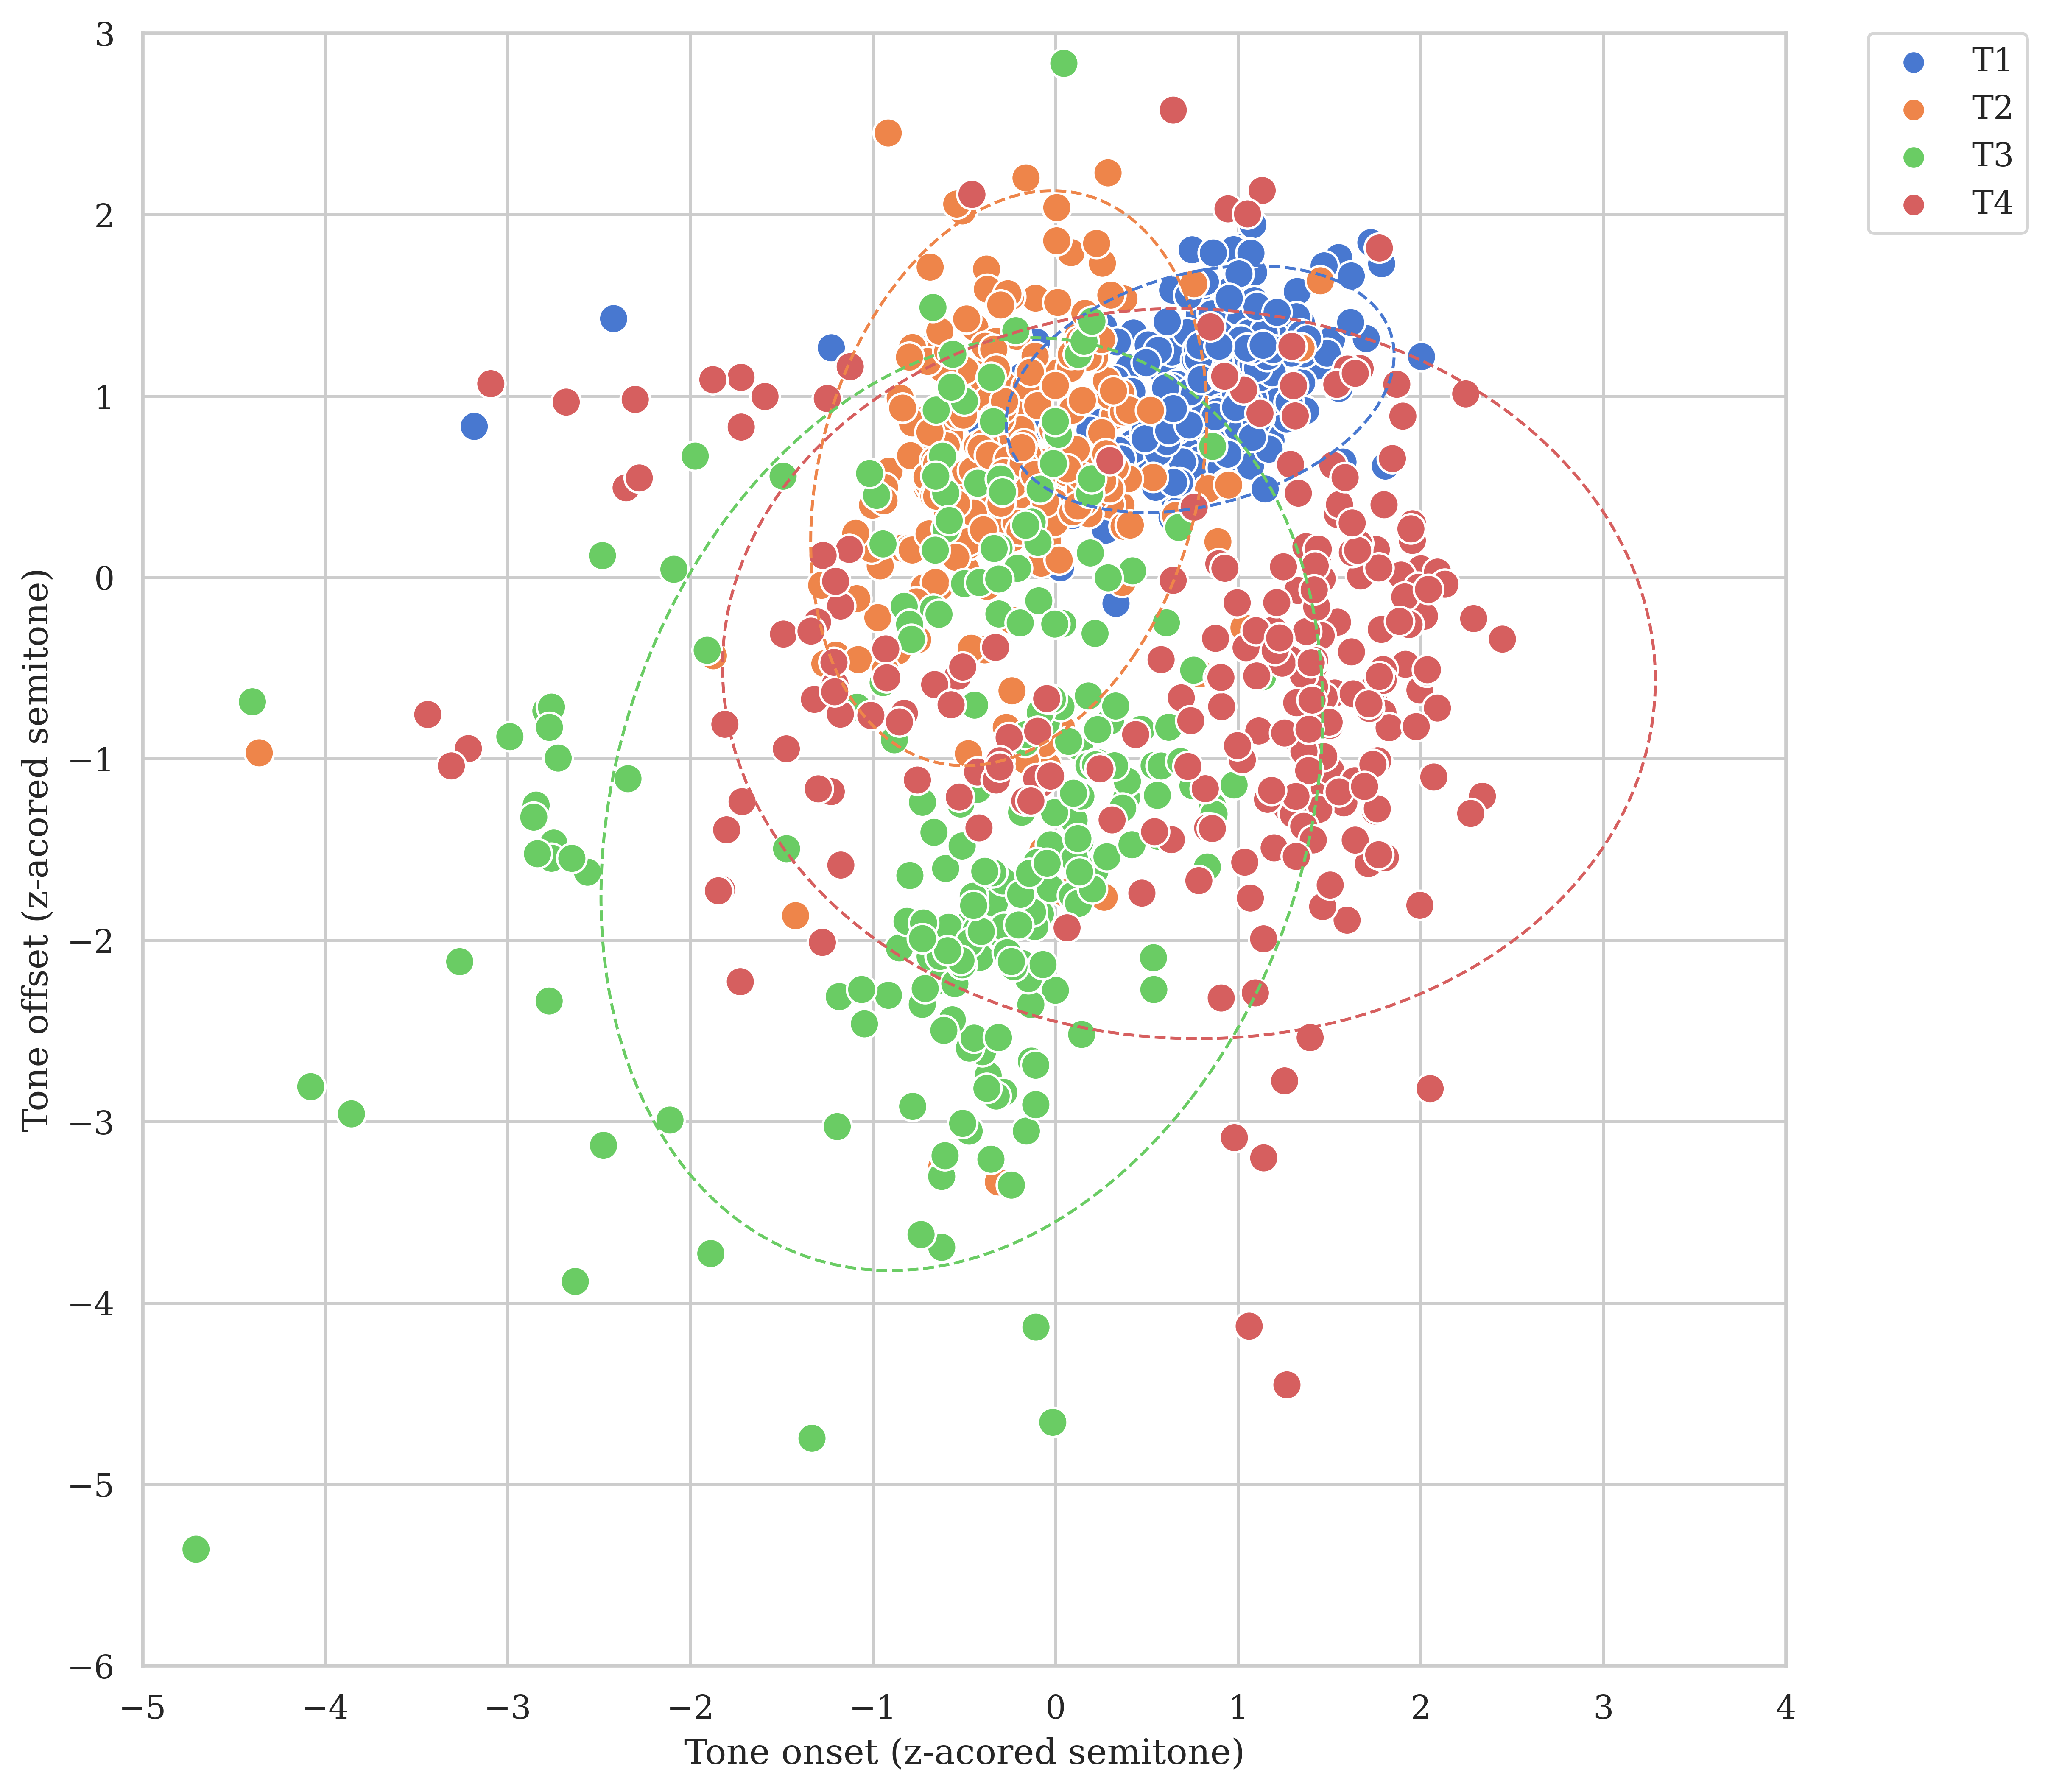
\includegraphics[width=\textwidth]{figures/Tone_space_Mandarin.png}
\end{subfigure}
\begin{subfigure}[b]{.8\textwidth}
\centering
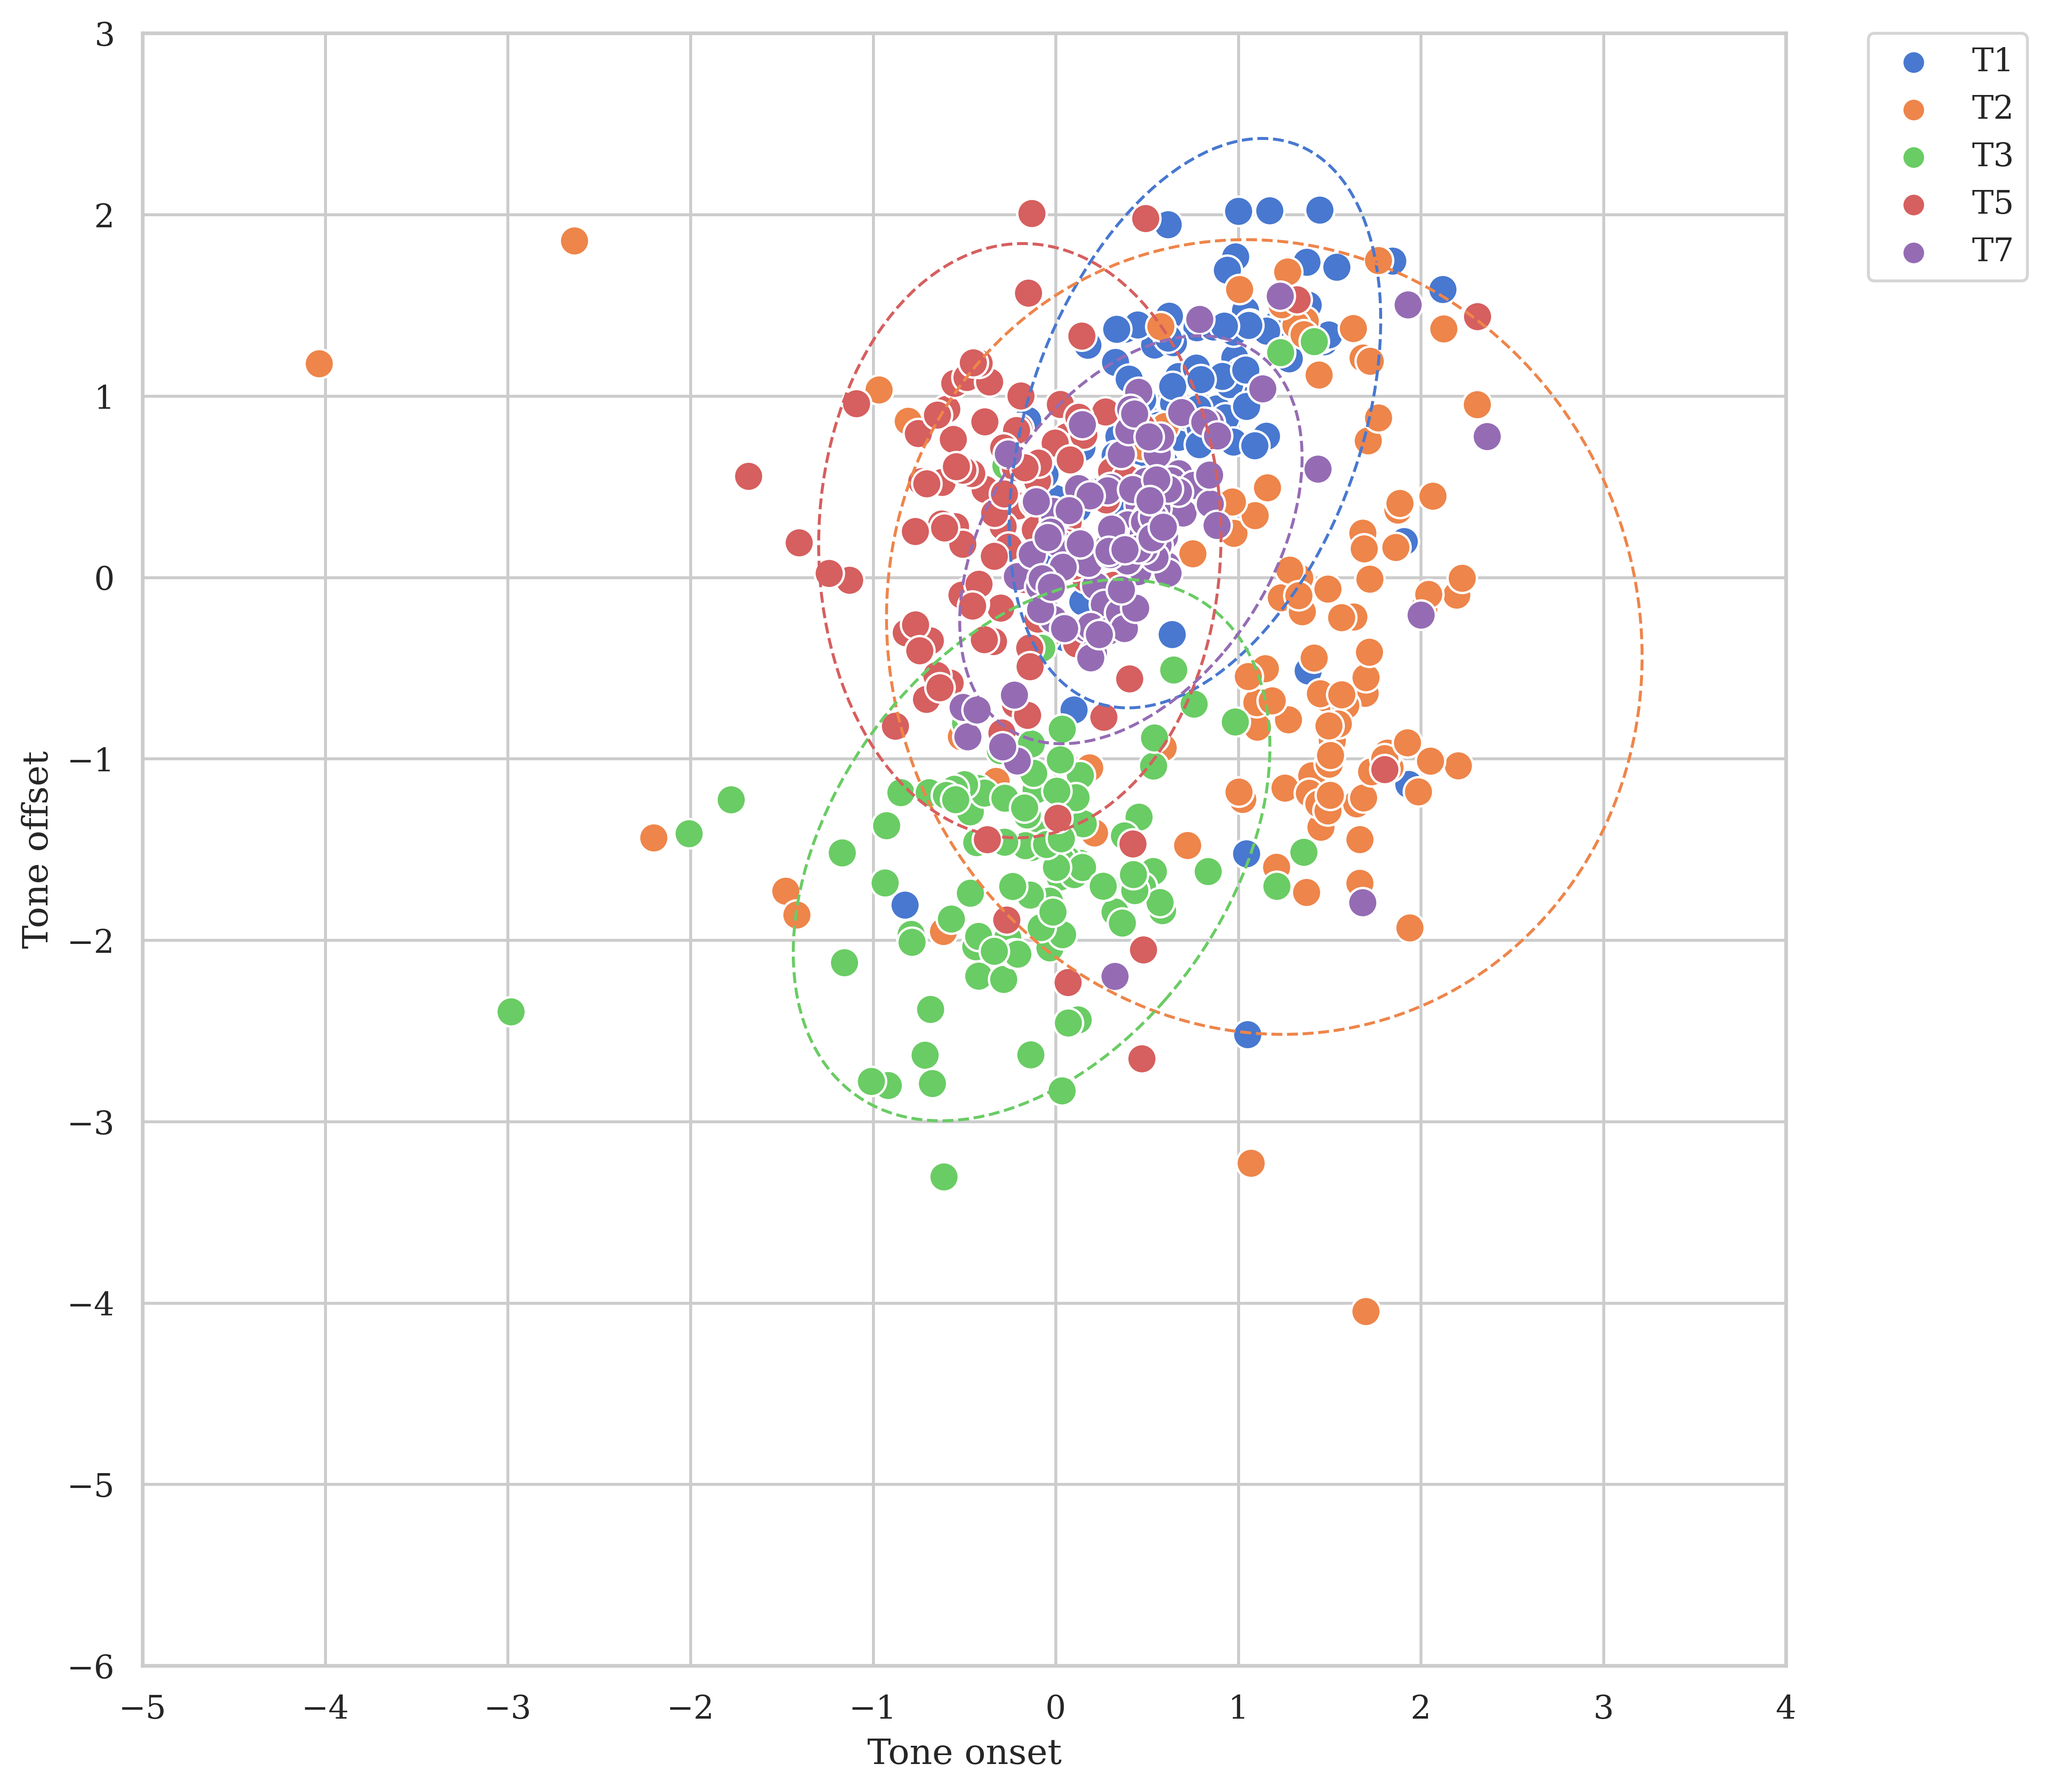
\includegraphics[width=\textwidth]{figures/Tone_space_Min.png}
\end{subfigure}

\caption{Tonal spaces of Taiwan Mandarin (top) and Taiwan Southern Min (bottom).}
\label{Figure:ToneSpace}
\end{figure}
It is imaginable that tone perception in Taiwan Southern Min would be challenging for listeners when tonal coarticulation is present. Recall that in Chapter \ref{chapter:Introduction}, three possible scenarios of tone perception under tonal coarticulation are discussed (cf. Figure \ref{Figure:ThreePossibleScenarios}). From the acoustic data in this study, scenario C, where the language has weak tonal coarticulation and the tones are directly identified without great perturbation seems invalid, as tonal coarticulation is of the same magnitude in Taiwan Southern Min as in Taiwan Mandarin. This leaves us with two possible scenarios. One is what we have seen in Mandarin (cf. \citealp{Zhangetal2022}), where strong normalization is attested. In both \cite{Xu1994} and \citeauthor{Zhangetal2022}, the perception of coarticulated tones was subject to normalization. Mandarin listeners, whether implicitly or explicitly, enlist the knowledge of pitch variation caused by adjacent tone's F0 values, and make according adjustment in order to retrieve the target that the interlocutor means to produce. While such account suffices to explain the perception of coarticulated tones, it cannot reconcile with the Taiwan Southern Min data we see in this study. In this study, Taiwan Southern Min, though having the same tonal coarticulatory effects as Taiwan Mandarin, has significantly weaker normalization effects. Just as mentioned in Chapter \ref{chapter:Introduction}, this result is understandable. If Taiwan Southern Min users are to rely only on normalization for tone identification under coarticulation, one would have much more possible candidates to normalize back to than in Taiwan Mandarin. (cf. perceptual recoverability in \citealp{Flemming2011}). The weaker normalization effect suggests some other factors are at work for Taiwan Southern Min speakers to facilitate effective communication. It is possible that Taiwan Southern Min is a language that takes on the route B in Figure \ref{Figure:ThreePossibleScenarios}, where the speakers have stricter tone boundaries for lexical tones. This scrutiny prevents coarticulated tones from being perceived as other lexical tones at the phonemic level. It is likely that, for Taiwan Southern Min listeners, a raised low tone that would be taken as an acceptable token of high tone in Taiwan Mandarin would be rejected, and still be perceived as a low tone. This can be illustrated in Figure \ref{Figure:ToneAcceptanceIllustration}. 
\begin{figure}[hbt!]
\centering
\begin{subfigure}[b]{.495\textwidth}
\centering
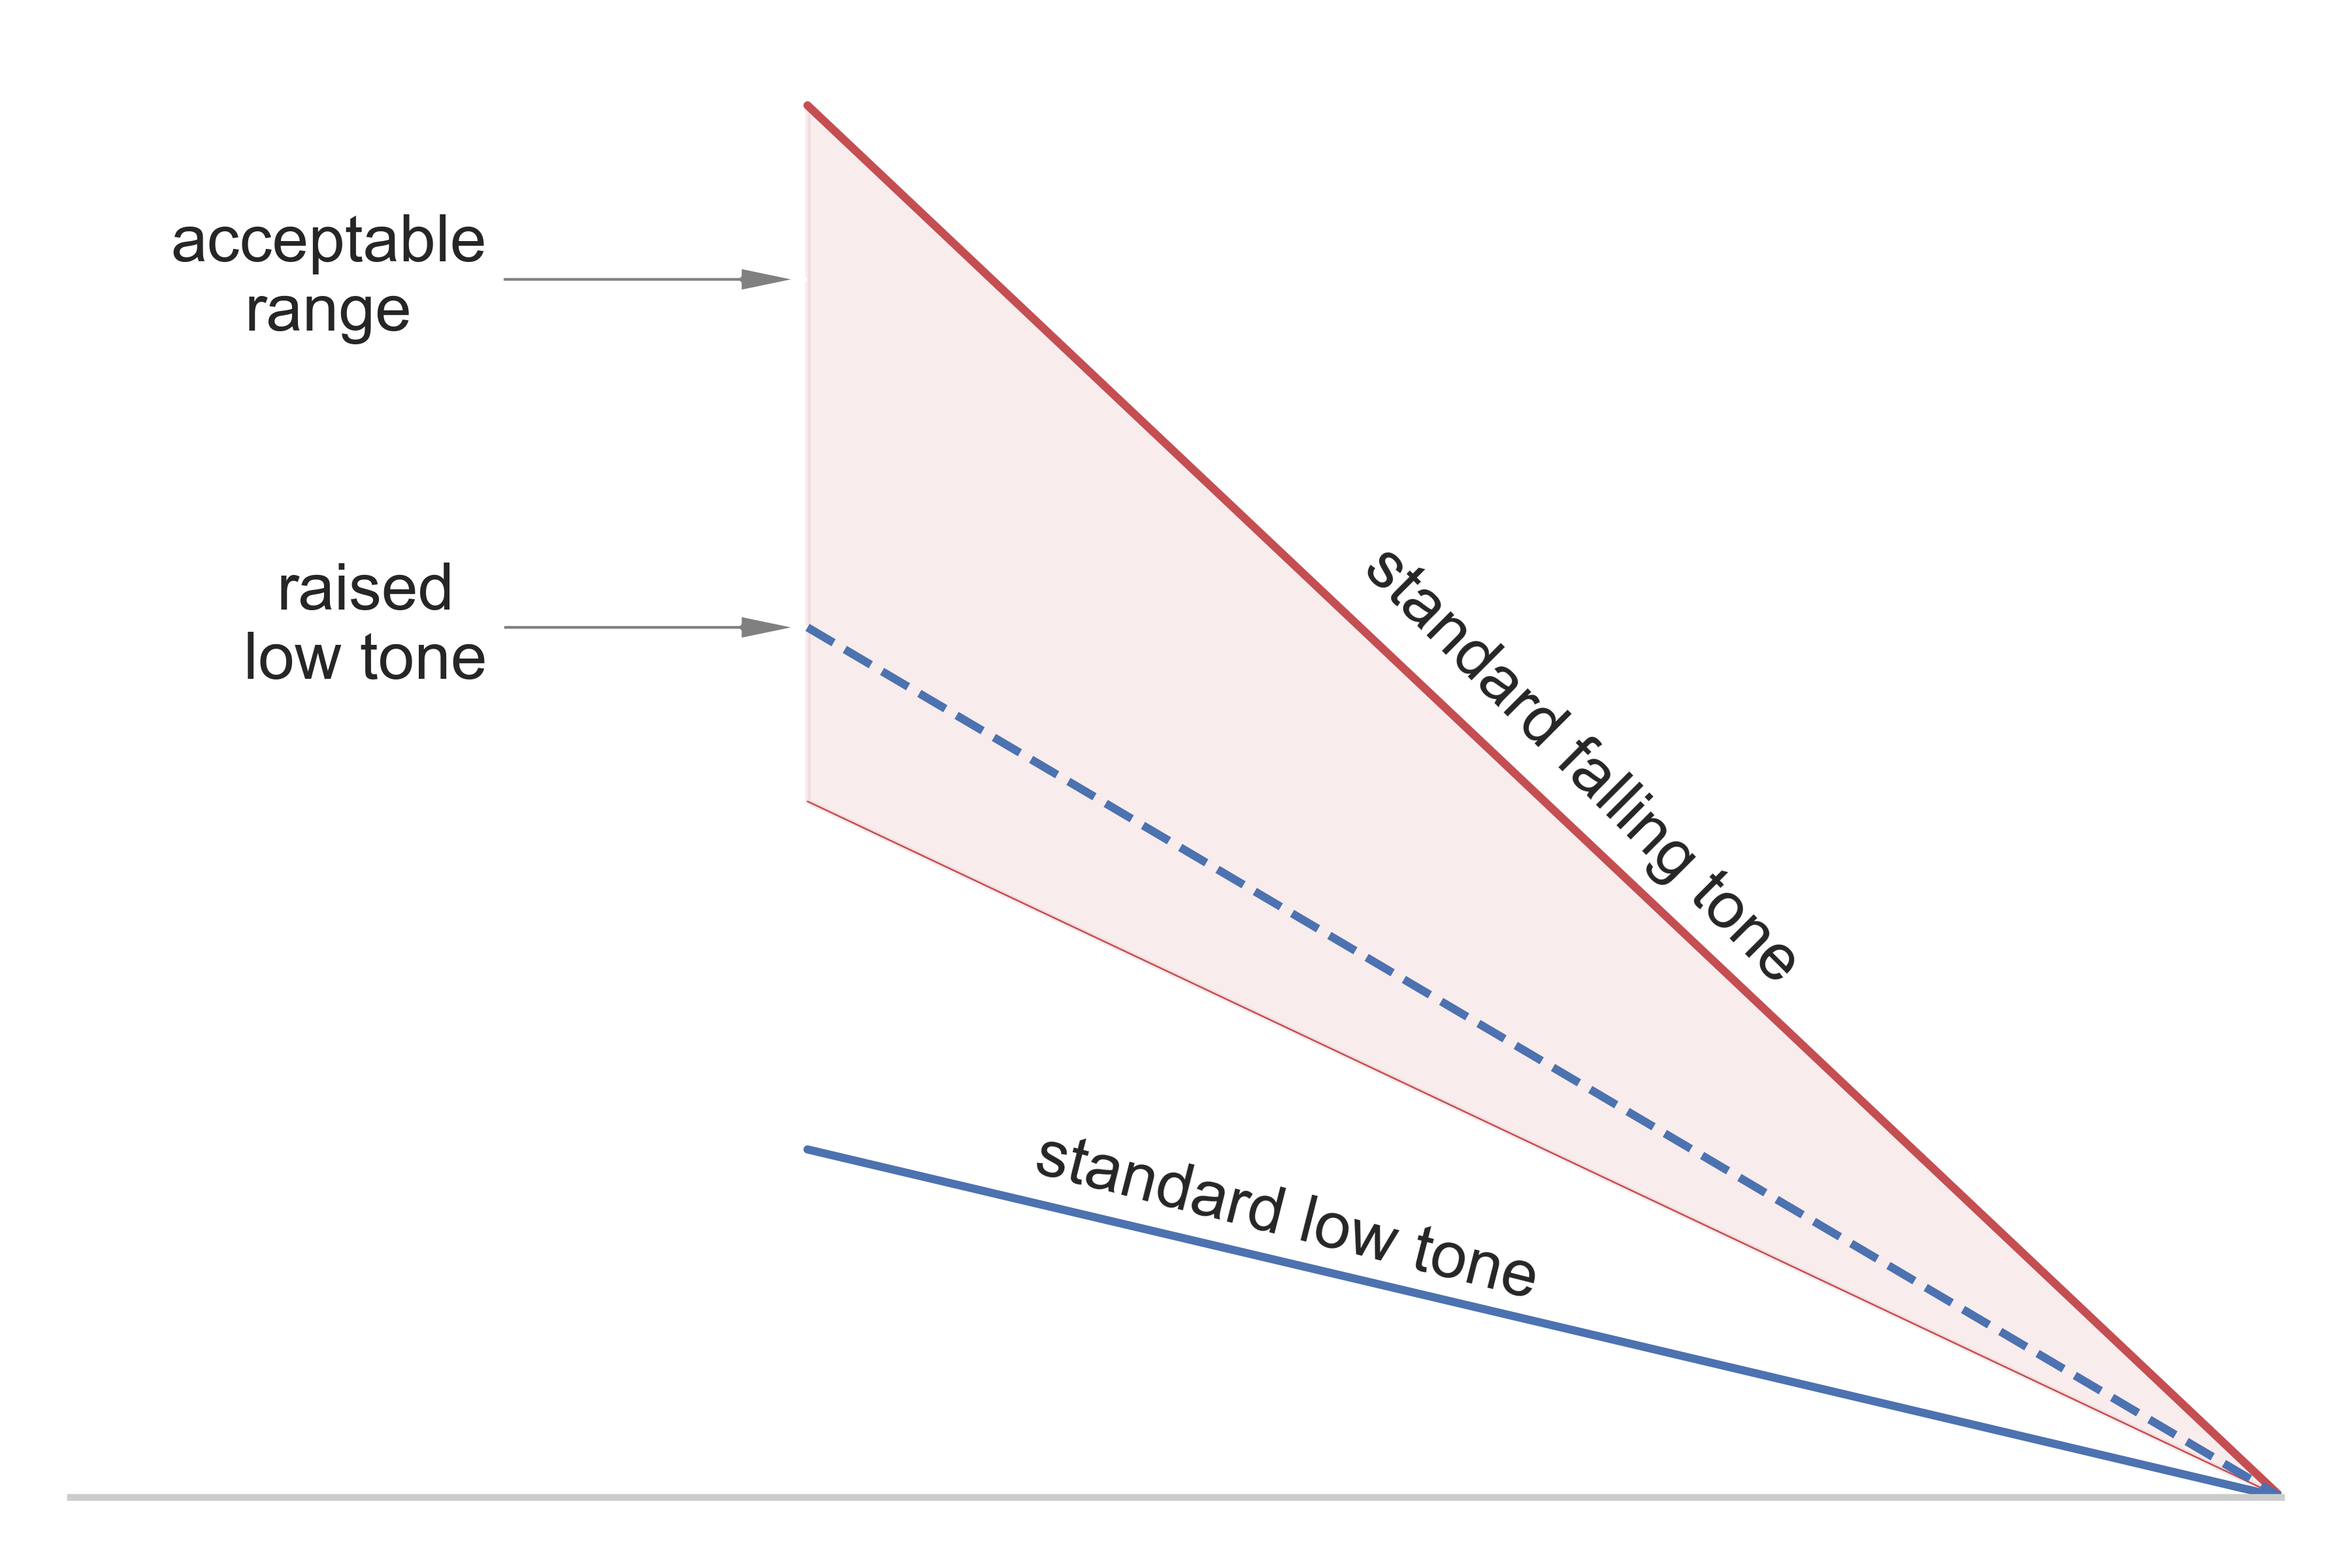
\includegraphics[width=\textwidth]{figures/Tone_acceptance_illustration_wide.png}
\end{subfigure}
\begin{subfigure}[b]{.495\textwidth}
\centering
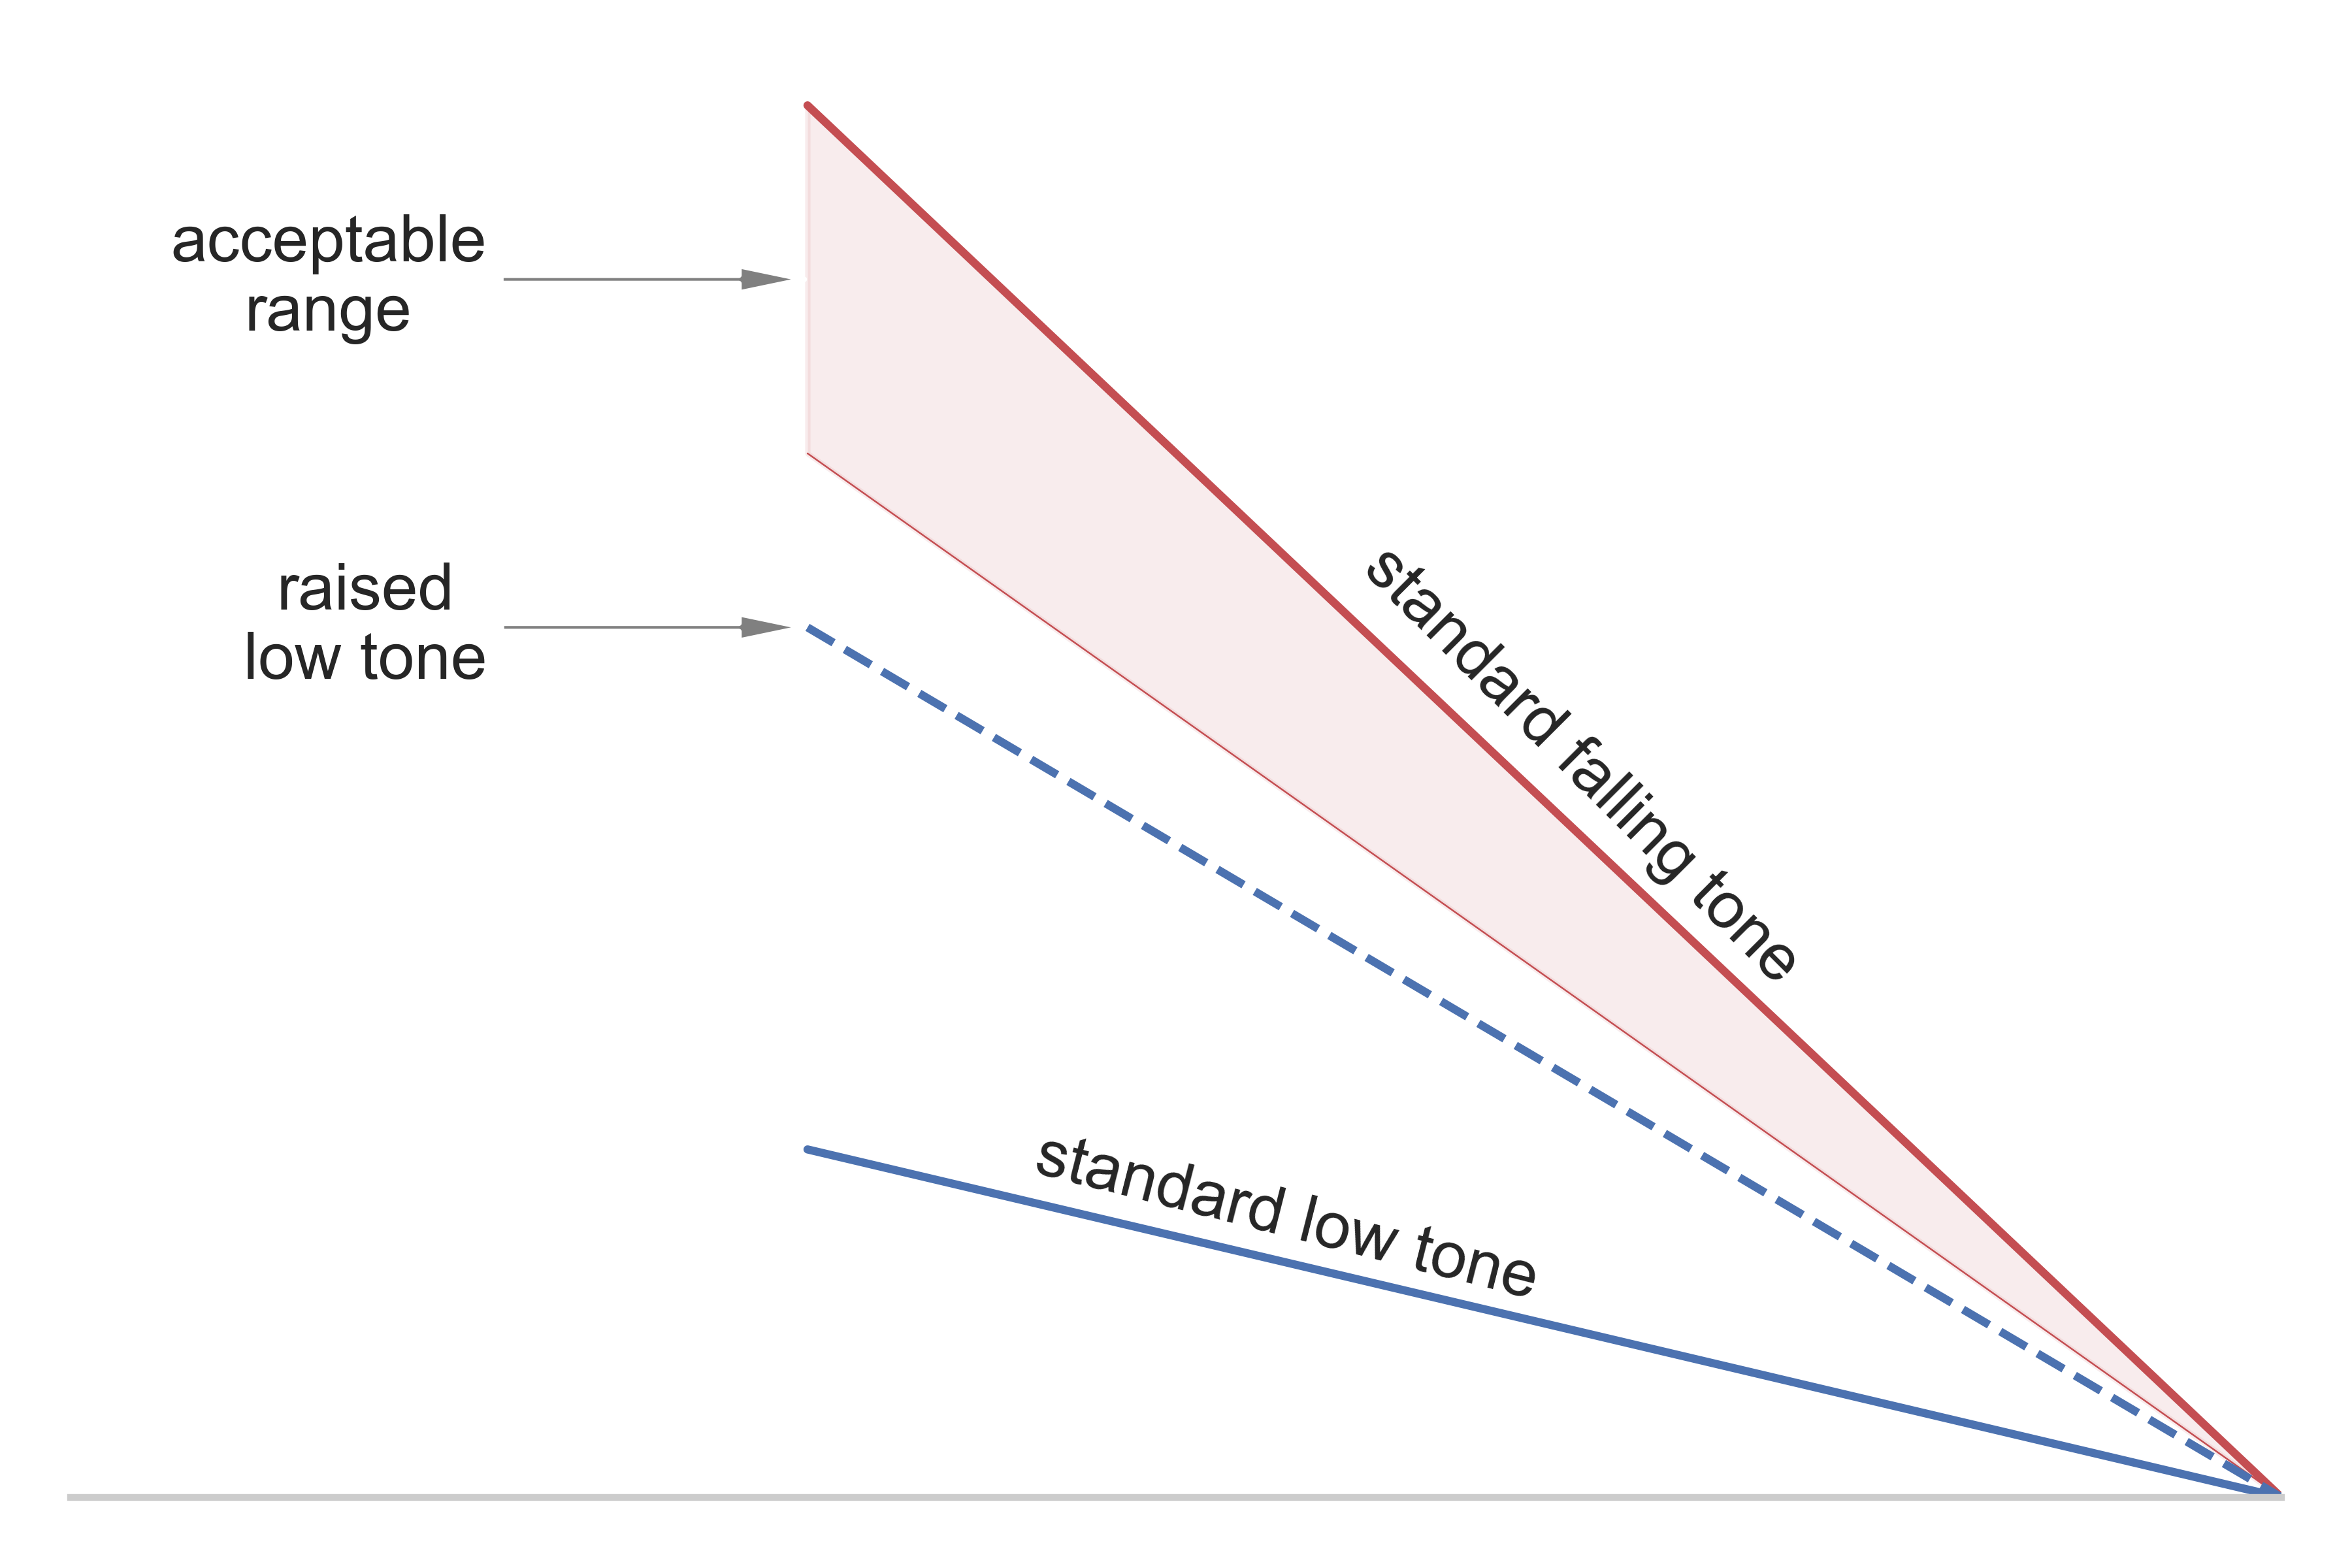
\includegraphics[width=\textwidth]{figures/Tone_acceptance_illustration_narrow.png}
\end{subfigure}

\caption{Illustrations of wider (left) vs. narrower (right) tone acceptance ranges.}
\label{Figure:ToneAcceptanceIllustration}
\end{figure}
In this case, normalization is less likely, since perceptually, the low tone is never a high tone to begin with. Indeed, if we look at the results of Experiment 3, we see that Taiwan Southern Min subjects had lower tolerances for Taiwan Southern Min falling tone than their Taiwan Mandarin counterparts did for Taiwan Mandarin falling tone. The question is why reversed was found for the low tones. For the low tones, the Mandarin subjects had steeper regression lines. This is likely due to the fact that under sandhi rules, Taiwan Southern Min low tone becomes the falling tone. Though the stimuli was isolated disyllabic words, and the subjects were reminded that the words were produced in isolation and therefore should not undergo sandhi changes, several subjects reported feeling both the low tone versions and falling tone versions to be acceptable for them. This might explain why the boundaries for the low tone were not significantly stricter for Taiwan Southern Min subjects as seen in the falling tone. That is to say, judging from the results seen in Experiments 2 and 3, Taiwan Southern Min differs from Taiwan Mandarin in that, though both have rather strong tonal coarticulation, the former has stricter tone boundaries that prevents coarticulated tones from being perceived as other lexical tones, while the latter accepts them as good tokens of other lexical tones, and undergoes normalization afterwards.

\section{The nature of tonal coarticulation}
After seeing tonal coarticulations in Taiwan Mandarin and Taiwan Southern Min, a question naturally arises: Is tonal coarticulation a universality that occurs naturally due to bio-mechanical or other phonetic factors? As argued in Chapter \ref{chapter:Introduction} and in the previous section, it is doomed to be painstaking for a language with large tone inventory to allow for tonal coarticulation. Perception becomes challenging with the already complicated tonal space becoming even messier, and normalization would also be hard considering the multiple possibilities of the target tone. As shown, Taiwan Southern Min listeners had to have stricter tone boundaries to attain successful comprehension. Things would be easier, if tonal coarticulation were absent or weaker. This is, nevertheless, not the case in Taiwan Southern Min. We see, instead, rather similar coarticulatory effects for both languages. This suggests that such effects might be involuntary, and conditioned by universal constraints. The linguistic discrepancy we see in past studies might well be the concomitant of lower-level language-specific grammar differences. Several studies have entertained this line of thinking. \cite{ShihSproat1992}, as afore-mentioned, found coarticulatory effects in Mandarin to be subject to prosody. This might help explain why symmetric results were found in \cite{Shen1990}'s Mandarin study. The requirement of the subjects to place the same duration and emphesis on the syllables might have effectively erased away the asymmetry seen in other studies led by the inherent rightward bias in Mandarin (\citealp{Hyman2007}). Likewise, \cite{Haoetal2018}, attempted to account for tonal coarticulation in Mandarin with articulatory effects. Varying results of coarticulated tones in continuous speech were modeled as factored by competition of attempt to decrease articulatory effects and the prosodic functional need due to requirements such as accentuation. This modeling was found to be capable of explaining the variations seen in Mandarin tonal coarticulation. In this case, the variations we see in coarticulated tones are merely byproducts of different prosodic needs. The authors also found that duration could help distinguishing tones with and without coarticulation. This hints that tonal coarticulation is likely influenced by biological mechanism. \cite{Flemming2011} also proposes that certain cross-linguistic universal constraints exist, and it is language-specific variations that interact with such constraints, resulting in the discrepancies we see in languages. While the nature of tonal coarticulation is not the direct tenet of this study. We should at least consider the possibility that tonal coarticulation might be to a certain extent universal across languages.

\section{General perceptual compensation vs. speech-specific normalization}\label{section:General perceptual compensation vs. speech-specific normalization}

Another issue that is, though not the main theme of this study, worth discussing is the debate over whether the normalization we have seen is linguistic or is merely part of the broader general perceptual compensation. This has been debated in past literature. People like \cite{WatkinsMakin1994} and \cite{Zhangetal2022} argue that what is generally believed to be speech-specific normalization can actually still be induced even when the stimuli are non-speech materials. This is what \citeauthor{Zhangetal2022} have found in their study, where higher/lower frequency non-speech stimuli could elicit similar effect in their experiment. However, this effect was significantly weaker than when the stimuli were speech sounds. Even the authors had to admit that linguistic factors had a role to play in what they called ``perceptual compensation''. In our study, linguistic differences were shown to have great effect on the outcome of normalization. Even when the two languages' stimuli had exactly the same F0 values, durations, and intensities, the two language groups showed different degrees of normalization. What strengthens this stance even more is the fact that both the linguistic differences seen in Experiments 2 and 3 are shown to be kept even within the same subjects, suggesting that such discrepancy cannot even be attributed to individual difference. This strongly urges one to believe that the phenomenon of normalization is not something common among cognitive systems, but is unique to the linguistic faculty.

\section{Sectional summary}
In this section, results of the experiments and their implications were discussed. Tonal coarticulation in Taiwan Mandarin and Taiwan Southern Min were found to be virtually identical, with both being symmetric and of similar magnitude. This dialectal discrepancy between Beijing and Taiwan Mandarins were attributed to Taiwan Southern Min's influence, in which tonal coarticulation has been found to be generally symmetric in several past studies. Taiwan Southern Min speakers were, nevertheless, found to exhibit normalizing effects to a lesser degree compared with their Taiwan Mandarin counterparts. Joined with the stricter tone boundaries seen in Experiment 3, it is believed that Taiwan Southern Min speakers reject coarticulated tones as good tokens of other lexical tones at the phonemic level, while Taiwan Mandarin speakers had looser acceptances, and retrieved the intended target tones by means of normalization afterwards.

The natures of tonal coarticulation and normalization are also addressed. It is believed that tonal coarticulation is in essence language-universal, and whatever difference attested among languages is highly likely concomitant of other linguistic specificities. Normalization is shown to be speech-specific, rather than cognitively general, due to the apparent discrepancy between Taiwan Mandarin and Taiwan Southern Min seen in Experiment 2.
